\documentclass[11pt,a4paper]{article}
\usepackage[T1]{fontenc}
\usepackage[utf8]{inputenc}
\usepackage{lmodern,microtype}
\usepackage[margin=26mm,headheight=15pt]{geometry}
\usepackage{amsmath,amssymb,amsthm,mathtools}
\usepackage{booktabs,longtable,array,enumitem}
\usepackage[dvipsnames]{xcolor}
\usepackage{graphicx,fancyhdr}
\usepackage{listings,xurl}
\usepackage[colorlinks=true,linkcolor=MidnightBlue,citecolor=MidnightBlue,urlcolor=MidnightBlue]{hyperref}
\usepackage[nameinlink,noabbrev]{cleveref}
\definecolor{ink}{HTML}{17354A}
\definecolor{teal}{HTML}{126C73}
\definecolor{pale}{HTML}{F2F5F7}
\hypersetup{pdftitle={Polynomial Projectors and Compressed Surface Assembly for Unknot Recognition},pdfauthor={Research continuation prepared with ChatGPT for Vladimir Reshetnikov}}
\pagestyle{fancy}\fancyhf{}
\fancyhead[L]{\small\color{ink}Unknot recognition: projectors and seams}
\fancyhead[R]{\small 8 October 2026}\fancyfoot[C]{\thepage}
\setlength{\parskip}{4pt}\setlength{\parindent}{0pt}
\setlist{topsep=5pt,itemsep=3pt,parsep=0pt}
\lstset{basicstyle=\small\ttfamily,breaklines=true,columns=fullflexible,keepspaces=true,backgroundcolor=\color{pale},frame=single,rulecolor=\color{pale},xleftmargin=4pt,xrightmargin=4pt}
\newtheorem{theorem}{Theorem}[section]
\newtheorem{proposition}[theorem]{Proposition}
\newtheorem{lemma}[theorem]{Lemma}
\newtheorem{corollary}[theorem]{Corollary}
\theoremstyle{definition}\newtheorem{definition}[theorem]{Definition}
\newtheorem{example}[theorem]{Example}
\theoremstyle{remark}\newtheorem{remark}[theorem]{Remark}
\newcommand{\F}{\mathbb F_2}
\newcommand{\Z}{\mathbb Z}
\newcommand{\N}{\mathbb N}
\newcommand{\End}{\operatorname{End}}
\newcommand{\im}{\operatorname{im}}
\newcommand{\id}{\operatorname{id}}
\newcommand{\rank}{\operatorname{rank}}
\newcommand{\poly}{\operatorname{poly}}
\newcommand{\code}[1]{\nolinkurl{#1}}
\newcommand{\bits}{\operatorname{bits}}
\newcommand{\mi}{\mathbin{-}}
\title{\vspace{-12mm}\color{ink}\textbf{Polynomial Projectors and\newline Compressed Surface Assembly}\\[5pt]\large Two certified decomposition kernels for the\newline ProveIt unknot-recognition program}
\author{Research continuation prepared for Vladimir Reshetnikov\\\small with ChatGPT; proofs, implementation, and reproducible checks}
\date{8 October 2026\\\small Repository baseline: \texttt{bc5b913850f78155ccfddd808d4b11517dca252d}}
\begin{document}
\maketitle
\begin{abstract}
We develop two exact improvements to the decomposition machinery in
\code{Topology/UnknotRecognition}. The algebraic improvement augments the
existing scalar Fitting splitter with polynomial idempotents obtained from
Berlekamp's Frobenius fixed algebra. It can expose direct summands when a
chosen chain endomorphism is invertible and its stable kernel is zero. All
matching, homological, and recovered quantum types are preserved, and every
transformed differential attachment is checked. An explicit connected family
of two-term graded complexes has scalar endomorphism algebra
$\mathbb F_{2^r}\times\mathbb F_{2^r}$. On a uniform candidate, the old
zero-eigenvalue test succeeds with probability
$2(2^r-1)/2^{2r}$, whereas the polynomial-projector test succeeds with
probability at least $1-r/2^r$. This is a separation between candidate tests,
not a claim about all search policies or about realizability by knot prefixes.

The geometric improvement assembles binary dihedral surface-cover patches
across verified full-boundary seams. A spanning-forest gauge reduces the
assembly to one dihedral monodromy problem per connected base component.
Component counts, orientability, genus, residual boundary lifts, and marked
sheet queries are computed in bit-polynomial time without enumerating the
sheets. Closed outputs and nonorientable seams are allowed. An annulus example
shows that identical local topology can assemble into two Klein bottles or one
torus solely because the seam shift changes.

The package contains an optional production primary-splitting backend, a
standalone geometric assembly API, independent checks, raw measurements, and a
pinned integration patch. Neither result supplies the missing global bound on
recognition states or hierarchy repairs. We give precise conditional cost
statements and a research agenda that separates these remaining obligations
from the operations now implemented.
\end{abstract}
\clearpage
\tableofcontents
\newpage

\section{Results, scope, and relation to the existing program}
\label{sec:scope}

The purpose of this continuation is to improve operations that can actually
occur inside a complete recognition strategy, while keeping their cost and
logical role explicit. The maintained code already combines structural
certificates, invariant filters, diagram simplification, and an exact
Khovanov fallback. It also contains experimental compressed algebra and
surface-cover infrastructure. Two gaps in that infrastructure are particularly
concrete: detecting scalar direct summands beyond the stable kernel of a
candidate endomorphism, and composing multiple compressed cover presentations
without discarding their attachments.

The main contributions of this package are as follows.
\begin{enumerate}
\item An implemented, certificate-checked extension of the scalar splitter.
The new recognition option is \code{backend="primary"}; the exact-rank CLI
option is \code{khovanov --primary}. Both preserve the standard default policy.
\item A fully specified family demonstrating why a polynomial projector can
succeed when a Fitting test fails, together with exact success probabilities
for uniform endomorphism sampling. This also distinguishes a weakness of a
particular test from a weakness of the entire search strategy.
\item A checked geometric input model for assembling surface covers, a proof
that a spanning-forest reduction preserves all monodromy, and a binary
algorithm for the resulting topology and attachment queries.
\item A precise account of which remaining parameters would have to be
bounded to obtain $n^{O(\log n)}$ recognition, supported by reproducible
positive and negative experiments.
\end{enumerate}

Berlekamp's fixed-space construction, including its treatment of repeated
irreducible factors, is classical \cite{berlekamp}. Covering-space monodromy is
also classical \cite{hatcher}. The new work here is their checked application
to these particular repository interfaces, the explicit comparison family,
and the implementation and validation of the resulting operations. We make
no claim that polynomial idempotents or spanning-tree gauges originate here.

\begin{center}
\begin{tabular}{p{.26\linewidth}p{.34\linewidth}p{.30\linewidth}}
\toprule
Object & What is established & Remaining limitation\\
\midrule
Typed scalar complex & Exact polynomial-projector splitting of a chosen endomorphism & Candidate selection and live matrix dimensions remain uncontrolled globally\\
Surface-cover assembly & Exact topology and marked-sheet queries for checked complete seams & Extraction from arbitrary normal cuts and embedded 3-manifold provenance are not supplied\\
Complete recognizer & An additional exact optional backend & No general quasipolynomial running-time theorem\\
Measurements & Reproducible bounded experiments and independent comparisons & They are not worst-case or average-case complexity proofs\\
\bottomrule
\end{tabular}
\end{center}

All statements about the baseline refer to the commit shown on the title
page, rather than a moving branch. The source inspected includes
\code{scalar_split.py}, \code{barcode_scan.py}, \code{surface_cover.py}, and the
corresponding maintained synthesis sections \cite{repo}. Prior incoming
reports already contain additional Jones and compressed-word work. This
article does not present those results as new.

\section{The complexity target and the available geometric framework}
\label{sec:landscape}

Throughout, $n$ denotes the number of crossings in an explicit validated knot
diagram. Binary surface multiplicities and explicit matrix dimensions are
separate parameters. We use ``quasipolynomial'' for
$\exp((\log(n+2))^{O(1)})$, and reserve the sharper expression
$n^{O(\log n)}=2^{O((\log(n+2))^2)}$ for that particular target.

This distinction matters even in the motivational literature. The March
2021 Oxford handout states the announced running time
$2^{O((\log n)^3)}$, and describes a route through hierarchies of length
$O((\log n)^2)$ with polynomially bounded surface complexity
\cite[slides 7 and 25]{lackenby-talk}. The sharper target
$n^{O(\log n)}$ would improve that displayed estimate. We consider both the
general quasipolynomial goal and this stronger possibility, without
identifying their exponents.

Lackenby's July 2026 preprint gives a hierarchy algorithm and bounds its
iteration count by $L(g+1)^L$, where $L$ is maximal hierarchy length and $g$
is maximal pattern complexity. Its Section 9 explicitly leaves the cost of
some operations insufficiently specified for a running-time estimate. Its
Theorem 14.4 gives polynomial-time compressed cutting in the number of
uniform-type handles and the logarithm of extended normal weight, including
parallelity-bundle base topology and vertical attachments
\cite[Proposition 9.1 and Theorem 14.4]{lackenby-hierarchy}.

The Agol--Hass--Thurston orbit machinery provides an established general
framework for doing normal-surface topology without expanding all normal
discs \cite{aht}. The seam algorithm below is a restricted, particularly
explicit arithmetic kernel; it is not a replacement for that general theory.
Similarly, recent surface-curve algorithms compute geometric intersection
numbers and isotopy of essential normal 1-manifolds in time polynomial in
surface triangulation size and logarithmic curve weights
\cite[Theorems 1.1--1.2]{lackenby-curves}. These provide natural neighboring
interfaces for future attachment transport.

For the algebraic branch, Khovanov homology detects the unknot
\cite{kronheimer-mrowka}. The maintained code uses its characteristic-two
rank formulation and existing exact/capped continuation machinery. A scalar
chain isomorphism preserves all additive continuations, so our new splitting
step can enter that machinery without introducing an additional knot-theoretic
recognition hypothesis. The issue is the cost of constructing and simplifying
the complex, rather than soundness of an accepted scalar decomposition.

The two new kernels should therefore be assessed on two scales. Locally,
their correctness and bit complexity are fully specified. Globally, their
usefulness depends on whether a recognition algorithm can discover their
input presentations economically and keep their dimensions and number of
calls under control. Section~\ref{sec:global} formulates that separation as
explicit inequalities.

\section{Typed scalar endomorphisms of a scanning complex}
\label{sec:typed}

\subsection{The input category and the permitted changes of basis}

Let $C$ be a finite chain complex in the additive characteristic-two
cobordism category used by the scanner. Each object has a frontier matching
$m$, a homological degree $h$, and a recovered relative quantum shift $q$.
Write its scalar type as $\tau=(m,h,q)$, and let $V_\tau=\F^{d_\tau}$ be the
multiplicity space of objects of that type. Put
\[
 D=\sum_\tau d_\tau,\qquad V=\sum_\tau d_\tau^2.
\]
Here $D$ is an explicit live object count, and $V$ is the number of scalar
matrix variables. Neither is automatically small as a function of $n$.

A scalar typed endomorphism is a tuple
$Q=(Q_\tau)_\tau$ with $Q_\tau\in\operatorname{Mat}_{d_\tau}(\F)$ satisfying
\begin{equation}\label{eq:commute}
 Qd=dQ.
\end{equation}
The equality is tested coefficient by coefficient in each relevant morphism
space. Distinct morphism coefficients must not be collapsed to their support
size or to one scalar. In particular, a coefficient encoded by the integer
one need not be the identity between different matchings.

When all entries of an invertible scalar matrix stay within a type, its
change of basis is a legitimate isomorphism in the original category.
Recovering $q$ first prevents a scalar isomorphism from mixing different
quantum shifts. The existing implementation uses the relation
\[
 q_v-q_u=p-c_{uv}+2\delta_{uv}
\]
for a nonzero homogeneous entry from $u$ to $v$, where the frontier has
$2p$ endpoints, $c_{uv}$ is its overlay-circle count, and $\delta_{uv}$ is the
dot degree. All relevant cycles are checked for consistency. We preserve
this existing restriction \cite{repo}.

\subsection{Why whole-component verification is necessary}

We work on a whole connected component of the undirected differential graph.
A projector on a convenient internal block need not commute with maps to
other blocks. If those attachments are omitted, splitting can change later
homology even when the internal matrix calculation is correct.

\begin{lemma}[Typed projector splitting]\label{lem:projector}
Let $E$ be a typed scalar endomorphism of $C$ satisfying $E^2=E$ and $Ed=dE$.
Then
\[
 C\cong \ker E\oplus\im E
\]
by a typed scalar chain isomorphism. Every additive continuation functor
preserves this direct sum and its chain isomorphism.
\end{lemma}
\begin{proof}
In each multiplicity space, $v=(v+Ev)+Ev$, the first term lies in $\ker E$,
and the second lies in $\im E$. Their intersection is zero because $E$ acts
as zero on its kernel and as identity on its image. The commutation relation
makes both subspaces invariant under the differential. Choose bases for
the two parts within each type and concatenate them. The resulting change
of basis is invertible, and its conjugated differential has no cross terms.
An additive functor sends the change of basis and its inverse to mutually
inverse maps and preserves the displayed direct-sum decomposition.
\end{proof}

The implementation checks exactly the content needed for this argument:
types, invertibility, the coefficientwise commutator, the transformed
entries, and absence of every cross term. It also records the original and
transformed rows when witness recording is enabled. A cache hit is not an
exemption from commutator and basis-change verification.

\subsection{The existing Fitting test}

For a candidate $Q$, the old method chooses a power of two $N$ at least the
largest type-block dimension. Then $\ker Q^N$ and $\im Q^N$ are stable and
form a direct sum. If both are nonzero, they define a valid decomposition.
The method is inexpensive for a useful nilpotent part.

However, an invertible $Q$ always has zero stable kernel. This says nothing
about whether $Q$ has two different nonzero primary factors. It also says
nothing about whether the full commutant $\End(C)$ contains an idempotent.
The new operation addresses the first limitation for the same candidate;
it does not claim to solve the second problem for every complex.

\section{Polynomial projectors from the Frobenius fixed algebra}
\label{sec:berlekamp}

Let $\mu_Q(t)$ be the minimal polynomial of the direct sum of the blocks
$Q_\tau$, and let $d=\deg\mu_Q\le D$. Evaluation gives an injective algebra map
\[
 A_Q=\F[t]/(\mu_Q)\longrightarrow\prod_\tau\End(V_\tau),\qquad
 [p]\longmapsto p(Q).
\]
Injectivity is precisely the minimal-polynomial property. Every image
commutes with the differential because $Q$ does.

\begin{theorem}[Berlekamp fixed algebra, used as a splitting test]
\label{thm:fixed}
Write
$\mu_Q=\prod_{j=1}^s f_j^{e_j}$ with distinct monic irreducible $f_j$.
Then
\[
 \mathcal B_Q=\{[p]\in A_Q:[p]^2=[p]\}
\]
is an $s$-dimensional vector space over $\F$. It contains a nonconstant
class exactly when $s\ge2$. Every class other than $0$ and $1$ gives a
nonzero, nonidentity typed projector $p(Q)$, hence a chain splitting.
\end{theorem}
\begin{proof}
The Chinese remainder theorem gives
$A_Q\cong\prod_j\F[t]/(f_j^{e_j})$. Each factor is local. An idempotent
$e$ in a local ring is zero or one: if $e$ is a unit then $e^2=e$ implies
$e=1$; otherwise $1-e$ is a unit and $e(1-e)=0$ implies $e=0$.
Thus the idempotents correspond exactly to binary vectors in $\F^s$.
In a commutative ring of characteristic two, $(u+v)^2=u^2+v^2$, so these
idempotents are indeed closed under addition and scalar multiplication.
Evaluation is injective, preserving zero, identity, multiplication, and
types. Finally apply Lemma~\ref{lem:projector}.
\end{proof}

The theorem, including repeated powers $e_j>1$, is part of the classical
Berlekamp method \cite[pp.~1854--1858]{berlekamp}. We give the proof to make
clear why no squarefree assumption and no algebraic extension of the
coefficient field is hidden in our use of it.

\subsection{A factorization-free implementation}

In the basis $1,t,\ldots,t^{d-1}$ of $A_Q$, the map
\[
 \Phi:[p]\longmapsto[p^2+p]
\]
is binary linear. Its $j$th column is the coefficient vector of
$t^{2j}+t^j$ modulo $\mu_Q$. We compute its nullspace by packed binary
elimination. The nullspace contains $1$; if its dimension is at least
two, at least one basis member is different from $0$ and $1$ and supplies
a projector. We do not need to factor $\mu_Q$ first.

The minimal polynomial is obtained from the first linear dependence in
\[
 I,Q,Q^2,\ldots,Q^D.
\]
For each power, the blocks are flattened into one binary vector of length
$V$. Elimination retains both a pivot vector and its polynomial expression.
The first dependence has leading coefficient one and is the minimal
polynomial: a lower-degree annihilator would be an earlier dependence.
Cayley--Hamilton guarantees a dependence by degree $D$.

The discovery path evaluates $p(Q)$ using its retained powers. A separate
positive-certificate checker evaluates the displayed polynomial by Horner's
rule, verifies an annihilating polynomial, checks the fixed-polynomial
identity, and squares the proposed matrix. This checker need not prove that
the supplied annihilator is minimal. For a positive certificate, actual
idempotence, nontriviality, and chain compatibility suffice.

\begin{remark}[What a negative result means]\label{rem:negative}
If $\dim\mathcal B_Q=1$, then $\mu_Q$ is a power of one irreducible and no
nontrivial polynomial in this $Q$ is idempotent. The ambient complex may
still split. For example, $Q=I$ on two identical direct summands has
$\mu_Q=t+1$, yet projection onto one summand is a perfectly valid
non-polynomial idempotent. A failed candidate therefore retains the exact
component and continues the bounded search.
\end{remark}

\subsection{A worked six-dimensional candidate}

Take
\[
 f=t^3+t+1,\quad g=t^3+t^2+1,\quad
 \mu=fg=t^6+t^5+t^4+t^3+t^2+t+1.
\]
Both cubics are irreducible over $\F$: neither has a root in $\F$.
The polynomial
\[
 p=t^4+t^2+t
\]
has residues $0$ modulo $f$ and $1$ modulo $g$. Consequently
$p^2=p\pmod\mu$. On $Q=C_f\oplus C_g$, where $C_f,C_g$ are companion
matrices, $p(Q)$ is projection onto the second three-dimensional summand.
The candidate $Q$ is invertible because $f(0)=g(0)=1$, so its ordinary
stable-kernel split is trivial. Conjugating both matrices by any invertible
binary change of basis preserves these conclusions while hiding the
coordinate decomposition.

\subsection{Elementary bit bounds}

\begin{proposition}[Cost of a chosen candidate]\label{prop:cost}
For typed binary blocks of total dimension $D$, the elementary implementation
finds a polynomial projector or proves that none exists in $\F[Q]$ in
$O(D^4)$ bit operations and $O(D^3)$ bits of auxiliary storage. Positive
projector verification is polynomial in $D$. These bounds exclude the
initial construction of the scalar endomorphism space and the differential
basis change.
\end{proposition}
\begin{proof}
One block-matrix product costs at most
$O(\sum_\tau d_\tau^3)\le O(D^3)$ elementary binary operations. There are at
most $D$ products to generate powers. Their packed vectors have length
$V\le D^2$, and eliminating at most $D+1$ such vectors costs
$O(D^2V)\subseteq O(D^4)$. Retaining $D$ vectors of length $V$ costs
$O(D^3)$ bits. The Frobenius matrix has dimension at most $D$, and its
construction and nullspace are within the same bound by ordinary polynomial
reduction and elimination. Polynomial evaluation and squaring also fit.
Packed Python integer operations may improve constants but are not counted
as constant-time operations on unbounded integers.
\end{proof}

If there are $E$ binary commutation equations in $V$ variables, ordinary
elimination has the conservative bound $O(EV^2+V^3)$; equation assembly and
morphism transformation must also be charged. The production caps on objects,
variables, candidates, and splits remain important for exactly this reason.
A spectral test should not be described as polynomial in the logarithm of
an unexpanded matrix dimension.

\subsection{Simultaneous primary refinement}

The full Berlekamp space also describes a finite refinement procedure. Starting
from the identity idempotent, refine a current idempotent $e$ by the pair
$ep_j$ and $e(1+p_j)$ for each fixed-space basis member $p_j$, discarding zero
pieces. These products remain orthogonal idempotents. In the Chinese
remainder coordinates, the procedure separates the $s$ distinct coordinates,
so at most $s$ nonzero final pieces remain. This is the classical simultaneous
factor-separation mechanism \cite{berlekamp}.

The current production path takes one projector and lets its existing
component recursion continue. It does not implement a special batched
all-primary basis change. Avoiding repeated construction of commutant
systems after a large spectral split is a concrete future optimization,
with a well-defined algebraic target.

\section{A connected comparison family and exact success probabilities}
\label{sec:family}

This section constructs valid scanner-category complexes rather than
assuming that arbitrary binary matrices arise during a knot scan. We will
explicitly leave the latter realization question open.

\subsection{The family}

Let $r\ge3$, choose distinct irreducible monic polynomials $f,g\in\F[t]$ of
degree $r$, and put $q=2^r$. On one matching with two arcs, choose its two
dot variables $x,y$ in
\[
 R=\F[x,y]/(x^2,y^2).
\]
Set $A_0=\operatorname{diag}(C_f,C_g)$ and let
\[
 S=\begin{pmatrix}I&E\\0&I\end{pmatrix},\qquad
 A=SA_0S^{-1}
   =\begin{pmatrix}C_f&C_fE+EC_g\\0&C_g\end{pmatrix},
\]
where $E$ is any nonzero rank-one $r\times r$ matrix, for example
$E=e_1e_1^{\mathsf T}$. Define the two-term complex
\begin{equation}\label{eq:family}
 C_{f,g}:\quad R^{2r}\xrightarrow{xI+yA}R^{2r}.
\end{equation}
There are no further differentials, so $d^2=0$ automatically. Every nonzero
coefficient has dot degree one, and the two homological layers have a
consistent difference of quantum shift two. Hence the scalar-type
restriction used by the production splitter permits the entire matrix in
each layer.

\begin{lemma}\label{lem:connected}
The differential graph of \eqref{eq:family} is connected, and its typed
scalar chain-endomorphism algebra is isomorphic to
$\mathbb F_q\times\mathbb F_q$.
\end{lemma}
\begin{proof}
The coefficient of $x$ in a chain-commutation equation forces the source
and target scalar matrices to agree. The coefficient of $y$ then says that
this common matrix commutes with $A$. The companion module of an irreducible
polynomial is a simple cyclic $\F[t]$-module with endomorphism field
$\mathbb F_q$. There are no nonzero homomorphisms between the two modules
because their annihilators are coprime. Thus the centralizer of $A_0$, and
therefore of $A$, is the displayed product of fields.

For connectivity, the $xI$ edges join the corresponding source and target
vertices. Within either companion block, the shift entries of the companion
matrix connect all indices through these edges. The off-diagonal block
$C_fE+EC_g$ is nonzero: if it were zero, $E$ would be a nonzero module map
between the two nonisomorphic simple modules. One of its $y$ edges therefore
joins the two already connected blocks. No cancellation with $x$ can remove
this edge, because $x$ and $y$ are independent coefficients.
\end{proof}

The complex is minimal in the sense that its differential coefficients lie
in the radical $(x,y)$. Its hidden scalar splitting is not merely deletion
of a scalar unit. This makes it a relevant stress model for the actual
category, although no assertion is made that it is a reachable reduced
prefix of a classical knot.

\subsection{Fitting and primary success on a uniform candidate}

Under the isomorphism of Lemma~\ref{lem:connected}, a uniformly sampled
scalar endomorphism is a pair $(a,b)\in\mathbb F_q^2$. Sampling is uniform
when independent fair binary coefficients are used for a complete
$\F$-basis of the commutant. This is a mathematical comparison model. The
production policy first tries a bounded list of basis vectors and then a
fixed-seed list of combinations, so its measured behavior must be reported
separately.

\begin{theorem}[Exact candidate-test separation]\label{thm:probability}
For a uniform candidate on $C_{f,g}$, the ordinary stable-kernel test has
success probability
\begin{equation}\label{eq:fittingprob}
 P_{\mathrm{Fit}}=\frac{2(q-1)}{q^2}.
\end{equation}
Let $I_2(d)$ be the number of monic irreducible polynomials of degree $d$
over $\F$. The polynomial-projector test has success probability
\begin{equation}\label{eq:primaryprob}
 P_{\mathrm{Prim}}=
 1-\frac{1}{q^2}\sum_{d\mid r}d^2I_2(d)
 \ \ge\ 1-\frac r q.
\end{equation}
Thus repeated independent Fitting trials need an expected
$q^2/(2(q-1))$ candidates. Repeated independent primary trials need at most
$(1-r/q)^{-1}$ candidates.
\end{theorem}
\begin{proof}
Multiplication by a nonzero field element is invertible, and multiplication
by zero is zero. A nontrivial stable kernel/image decomposition therefore
occurs exactly when one of $a,b$ is zero and the other is nonzero, giving
\eqref{eq:fittingprob}.

The minimal polynomial of the direct-sum action is the least common
multiple of the minimal polynomials of $a$ and $b$. Each individual
minimal polynomial is irreducible. Consequently the Berlekamp dimension
is one exactly when $a$ and $b$ have the same minimal polynomial. An
irreducible of degree $d$ has all its $d$ distinct roots in $\mathbb F_q$
exactly when $d\mid r$. Its contribution to the number of ordered pairs
with the same minimal polynomial is $d^2$. This proves the equality in
\eqref{eq:primaryprob}. For each $a$, its Frobenius orbit contains at most
$r$ possible $b$, giving at most $rq$ failing pairs and the inequality.
Expected trial counts follow from the geometric distribution.
\end{proof}

The separation is exponential in $r$ for the \emph{number of independent
candidate tests}. It is not automatically an exponential end-to-end
speedup: constructing the commutant, the relative per-candidate costs, and
the possibility that a deterministic basis vector already splits must all
be counted. The elementary costs above are polynomial in $r$, so the
uniform-sampling comparison still gives an exponential expected-cost
separation for these two isolated test strategies once their common
commutant has been supplied. Section~\ref{sec:experiments} separately records
the actual bounded policy.

\subsection{A universal information limit of one candidate}

The product-field family is favorable because its two field values usually
have different minimal polynomials. If several summands receive Frobenius
conjugate values, the same polynomial $p$ cannot distinguish them: evaluation
in $\F[Q]$ sees only primary factors, not an independently labeled copy of
each summand. This is a structural limitation of every polynomial-in-one-
endomorphism scheme, not a numerical failure. Additional candidates or
noncommutative commutant information are required for those collisions.

Conversely, an accepted projector is useful even if it does not expose every
indecomposable summand. Literal component sharing and interval normalization
may benefit from a partial split. The new method therefore composes with the
existing exact operations rather than replacing their correctness arguments.

\section{A checked input model for assembling compressed surface covers}
\label{sec:seam-input}

\subsection{Pieces, canonical peripheral systems, and binary fibres}

A piece is a connected compact surface $F_v$ with nonempty boundary, given by
its orientability, genus or crosscap number, and number $b_v$ of boundary
components. A canonical polygon schema supplies a free generating system
for $\pi_1(F_v)$, an orientation bit for each generator, and based peripheral
words for its boundary circles. An orientable genus-$g_v$ piece has free rank
$2g_v+b_v-1$; a nonorientable piece with $k_v$ crosscaps has rank
$k_v+b_v-1$. Handle generators have orientation bit zero, crosscap generators
have bit one, and peripheral generators have bit zero.

In this section every piece has the same sheet set
\[
 X=\Z/W\Z,\qquad W\ge1,
\]
with $W$ encoded in binary. Each free generator acts as an affine permutation
\begin{equation}\label{eq:affine}
 g(x)=s x+a\pmod W,\qquad s\in\{1,-1\}.
\end{equation}
Since the fundamental group of a bordered surface is free, any assignment
of these maps to its free generators defines a covering. The boundary
monodromies $B_{v,j}$ are then \emph{derived} from the canonical peripheral
words. The caller cannot supply unrelated boundary maps together with a
claimed genus and expect the kernel to certify a surface.

The covering of a piece can be disconnected. A connected component of the
piece-adjacency graph will ultimately have an ordinary degree-$W$ covering
over its connected sewn base surface, possibly with many connected covering
components. Different adjacency components can be processed independently.
The current API chooses one common $W$ for the whole request; varying $W$
across independent requests is immediate. Unequal sheet counts across a seam
are outside the interface.

\subsection{Seams and their exact compatibility condition}

A seam $e$ uses two distinct, previously unused boundary components
$(u,a)$ and $(v,b)$. The pieces $u,v$ may be equal. The seam specifies:
\begin{itemize}
\item a base boundary homeomorphism of degree $\varepsilon_e\in\{1,-1\}$;
\item a fibre bijection $A_e(x)=s_ex+a_e\pmod W$.
\end{itemize}
Boundary circles have fixed based parametrizations; the base map is the
canonical based map of degree $\varepsilon_e$, or a map in the same based
isotopy class. The seam joins the \emph{entire} inverse image of the first boundary to the
entire inverse image of the second. Every lifted circle participates. Its
necessary and sufficient compatibility check is
\begin{equation}\label{eq:seam}
 A_e B_{u,a}=B_{v,b}^{\varepsilon_e}A_e
 \qquad\text{as permutations of }X.
\end{equation}

\begin{lemma}[Realization of a seam]\label{lem:seam}
Condition~\eqref{eq:seam} is equivalent to existence of an isomorphism of
these complete boundary covers lying above the prescribed degree-$
\varepsilon_e$ base map and inducing $A_e$ on the reference fibre. Compatible
seams assemble the piece coverings into an unbranched covering of the sewn
surface, including when that surface is closed.
\end{lemma}
\begin{proof}
Represent a boundary covering by $X\times\mathbb R$ with
$(x,t+1)\sim(Bx,t)$. Following a once-around base loop before or after the
proposed fibre map must agree, which gives~\eqref{eq:seam}. Conversely the
map $(x,t)\mapsto(A_ex,\varepsilon_e t)$ respects these identifications
exactly when~\eqref{eq:seam} holds. It therefore descends to the required
circle-cover homeomorphism and induces $A_e$ at the reference fibre $t=0$.
Gluing collars along these
homeomorphisms gives covering charts across the seams; away from them the
original covering charts remain. Since each boundary is used once, the
quotient base and covering are surfaces and no branching is introduced.
\end{proof}

Two formal affine pairs need not be distinct permutations when $W$ is small.
The precise equality test is
\begin{equation}\label{eq:map-equality}
 (s,a)=(t,b)\text{ on }X
 \iff s-t\equiv0\pmod W\ \text{ and }a-b\equiv0\pmod W.
\end{equation}
Necessity follows by evaluating at zero and one; sufficiency follows by
subtraction. For $W=1$ every map is identical, and for $W=2$ the signs $1$
and $-1$ coincide as permutations. The code checks~\eqref{eq:map-equality}
rather than insisting on equality of the written signs. Otherwise it would
reject valid one- and two-sheet gluings.

\subsection{Orientation is additional data}

The sign $s_e$ of a fibre permutation is not a surface-orientation character.
These are independent quantities. Choose a local surface orientation at each
piece basepoint and fixed whiskers to its boundary reference points. Orient
each boundary using that transported local orientation. In this convention,
traversing a seam changes the transported surface orientation by
\begin{equation}\label{eq:seam-orientation}
 \sigma_e=[\varepsilon_e=+1]\in\F.
\end{equation}
An orientation-reversing identification of induced boundary directions
extends the same surface orientation over the seam, while an
orientation-preserving one requires its reversal. This explains the
indicator in~\eqref{eq:seam-orientation}.

For a nonorientable piece the canonical polygon schema still fixes the
whiskers and the local orientation choices. Orientation character on a
based loop is well defined even though a global orientation does not exist.
The implementation retains the character through every gauge change.

\section{Spanning-forest reduction and attachment-preserving monodromy}
\label{sec:gauge}

Let $\Gamma$ be the multigraph whose vertices are pieces and whose edges are
seams. Loops and parallel edges are allowed. Choose one root and a spanning
tree in each connected component. For a piece $v$, let $P_v$ be the fibre
transport from its root along the chosen tree path, and let $t_v\in\F$ be
the corresponding orientation-transport bit. Set $P_r=\id$ and $t_r=0$.
For a forward tree edge $u\to v$,
\[
 P_v=A_eP_u,\qquad t_v=t_u+\sigma_e.
\]
For a reversed tree traversal use $A_e^{-1}$; the same $\sigma_e$ applies.
All $P_v$ remain affine maps with sign $\pm1$, irrespective of the path's
length or the sheet count.

Transporting everything to the root yields the following data:
\begin{align}
 \widehat g_{v,i}&=P_v^{-1}g_{v,i}P_v,
 &\widehat\omega_{v,i}&=\omega_{v,i},\label{eq:localgauge}\\
 H_e&=P_v^{-1}A_eP_u,
 &\eta_e&=t_u+\sigma_e+t_v\quad(e\text{ non-tree}),\label{eq:seamgauge}\\
 \widehat B_{v,j}&=P_v^{-1}B_{v,j}P_v
 &&((v,j)\text{ unsewn}).\label{eq:boundarygauge}
\end{align}
Products mean composition, with the rightmost map acting first.

\begin{theorem}[Monodromy of the assembled cover]\label{thm:gauge}
For each connected component of $\Gamma$, the action on the root fibre
generated by~\eqref{eq:localgauge} and~\eqref{eq:seamgauge}, with their
displayed orientation bits, is the monodromy and orientation character of
the assembled surface covering. Its orbits are exactly the covering
components. Formula~\eqref{eq:boundarygauge} gives the residual peripheral
monodromies. A point in piece $v$ with local sheet $x$ belongs to the root
orbit of $P_v^{-1}(x)$.
\end{theorem}
\begin{proof}
Consider a loop in the sewn surface. Subdivide it whenever it crosses a seam.
Within a piece, replace each segment by the fixed whiskers and a word in the
piece generators. Insert tree paths from and back to the root between these
segments. The tree transports cancel in consecutive products. The remaining
root loops are generated by the conjugated piece loops and non-tree seam
loops, with precisely the fibre actions displayed above. Conversely every
listed generator is represented by such a based loop in the sewn surface.
This proves equality of the monodromy groups, not just one inclusion.

Orientation bits add along paths. A conjugated local loop contributes
$t_v+\omega_{v,i}+t_v=\omega_{v,i}$. A non-tree loop contributes
$t_u+\sigma_e+t_v$. The peripheral and point formulas are the same root-path
calculation. The standard monodromy correspondence identifies connected
covering components with orbits of the root fibre.
\end{proof}

This proof can be viewed as an explicit groupoid form of the classical
covering-space action construction \cite[Section 1.3]{hatcher}. It avoids
rewriting the sewn surface into a new canonical polygon, a step that could
otherwise discard useful labels or introduce large words.

\subsection{Closed bases are handled by actual gluing}

Once all boundaries are sewn, the base may be closed and its fundamental
group is generally no longer free. We do not assert that an arbitrary list
of affine maps defines a closed-surface covering. Instead, Lemma~\ref{lem:seam}
already constructs the covering. The relations of the closed base are
therefore automatically satisfied by the assembled action. This is the
reason the new kernel can safely extend the older bordered-cover interface
to closed outputs.

For each connected base component $F$, Euler characteristic is
\begin{equation}\label{eq:basechi}
 \chi(F)=\sum_{v\in\Gamma_F}\chi(F_v).
\end{equation}
Gluing circles changes no Euler characteristic. If $C$ is a connected
covering component of degree $d_C$, lifting a cell decomposition gives
\begin{equation}\label{eq:coverchi}
 \chi(C)=d_C\chi(F).
\end{equation}
Boundary counts and orientability then determine genus. These formulas
count actual covering degrees and topological characteristics; neither
multiplicities nor Euler characteristics are reduced modulo two.

\subsection{A replayable gauge certificate}

The assembly stores a record for every piece: its root, parent, tree seam,
traversal direction, affine transport, and orientation bit. An independent
checker validates the original seam equations, verifies every parent edge
and transport recurrence, rejects cycles, and checks that all seams stay
within the claimed forest components. Parent chains are settled once rather
than re-walked independently from each vertex.

This checker certifies the gauge reduction. It deliberately does not accept
an arbitrary serialized genus or component count as a verified topological
answer. The prepared index is reconstructed from the validated input; the
arithmetic classifier then computes its summary. Independent expanded-sheet
audits provide a separate implementation check on small inputs.

Changing the chosen root or tree changes coordinates but not the assembled
cover. The verifier accepts a valid alternative tree certificate. The
production index nevertheless retains its own normalized presentation and
labels, so its equality keys are defined within that presentation rather
than claiming to solve isomorphism of arbitrary surface decompositions.

\section{Exact orbit, orientation, and marking arithmetic}
\label{sec:orbits}

The root generators still have the form $x\mapsto\pm x+a\pmod W$.
We now recall and justify the arithmetic classification needed after
assembly. This is the extension point at which the existing dihedral
cover kernel is reused \cite{repo}.

\subsection{Translation-generated subgroup and component families}

If every generator has positive sign, set
\[
 d=\gcd(W,a_1,\ldots,a_k),\qquad m=W/d.
\]
The translation subgroup is generated by $T(x)=x+d$. Its orbits are the
$d$ residue classes modulo $d$, each of size $m$.

If reflections occur, choose one $R(x)=-x+a_0$. Define $H$ as the subgroup
generated by all displayed positive shifts and all products of two
displayed reflections. Its translation shifts are generated by the
positive shifts and the differences $a_i-a_0$ for the other reflections.
Take their gcd with $W$ as $d$ and again let $m=W/d$.
Products of two reflections give these differences, and conjugating a
translation by a reflection negates it. Bezout's identity proves that these
listed translations generate exactly $d\Z/W\Z$, so $H=\langle T\rangle$
and the full action is generated by $H$ and $R$. For $W\ge3$, $H$ is the
usual translation subgroup of that action. For $W\le2$, formal signs are
auxiliary labels and $H$ need not contain every group element that happens
to act as a translation; the displayed generation statement remains valid.

The reflection acts on residue classes modulo $d$ by
$r\mapsto a_0-r$. Let
\[
 f=\#\{r\pmod d:2r\equiv a_0\pmod d\}.
\]
This number is zero, one, or two. There are $(d-f)/2$ paired-residue
components of degree $2m$, together with $f$ fixed-residue components of
degree $m$. Thus at most three family records are required.

\begin{proposition}[Uniform family bound]\label{prop:families}
For each connected sewn base component, the assembly has at most three
component-family records, with multiplicities and covering degrees written
in binary. All paired-residue components are isomorphic as unmarked covers
of that fixed base. If two fixed-residue components occur, they are
isomorphic exactly when $m$ is odd.
\end{proposition}
\begin{proof}
Only the last two statements need explanation. For nonfixed residues $r,s$,
map the two translation orbits by
\[
 r+jd\mapsto s+jd,\qquad
 a_0-r+jd\mapsto a_0-s+jd.
\]
The resulting bijection commutes with $T$ and $R$, hence with all root
generators. For two fixed residues, an equivariant map must commute with the
transitive translation action and is therefore a translation. Their residue
difference is $d/2$ modulo $d$, so the translation has size $d/2+dt$.
Commutation with $R$ requires $2t=-1\pmod m$, which is solvable precisely
when $m$ is odd.
\end{proof}

The bound is per connected base component. A disconnected base with $k$
components can require up to $3k$ records. An unmarked isomorphism type is
also different from a particular component label: attachment queries must
retain which residue class or pair is selected, even when two selected
components happen to be isomorphic.

\subsection{Orientation through a character-consistency calculation}

Attach a bit $\omega(g)$ to each root generator. Write every translation
generator as a shift $a_j$ with bit $\beta_j$, and write the chosen
reflection as $(R,\beta_0)$. A product of two reflections supplies the
translation shift difference with the sum of their bits.

Use extended gcd to compute $d$ as an integer combination of $W$ and the
translation shifts. Applying the same coefficients modulo two to the
$\beta_j$ gives a candidate bit $\tau$ for translation by $d$. The orientation
character on the displayed translation words descends consistently to
$H$ exactly when
\begin{equation}\label{eq:consistency}
 m\tau=0\pmod2,\qquad
 \beta_j=(a_j/d)\tau\pmod2\quad\text{for every translation generator.}
\end{equation}
If these fail, an orientation-reversing identity translation exists; it
fixes every sheet, and every component is nonorientable.

Suppose~\eqref{eq:consistency} holds. A translation-only component is
orientable. A paired-residue component is also orientable: a reflection
changes residue classes and cannot stabilize a sheet; every stabilizing
translation has bit zero. On a fixed residue class $r$, a reflection
stabilizer is
\[
 T^{(2r-a_0)/d}R,
\]
whose orientation bit is
\begin{equation}\label{eq:fixedorientation}
 \beta_0+\frac{2r-a_0}{d}\tau\pmod2.
\end{equation}
That component is orientable exactly when this bit is zero.

These criteria remain valid when formal affine signs act nonfaithfully for
$W=1,2$. They inspect orientation bits of the actual stabilizers rather than
assuming that a written reflection has a nontrivial permutation action.
The repeated use of integer relations in~\eqref{eq:consistency} also explains
why an arbitrary choice of a gcd representative cannot silently change the
answer.

\subsection{Residual boundary-cycle profiles}

A remaining base boundary has a root affine monodromy $B$. If
$B(x)=x+a$, then $d\mid a$. On one translation orbit of size $m$, it has
\[
 c=\gcd(m,a/d)
\]
cycles, each of degree $m/c$. On a paired-residue component, there are two
such translation orbits, so the multiplicity doubles.

If $B(x)=-x+a$, then on a paired-residue component every cycle has length
two, with $m$ cycles. On a fixed residue $r$, its action in the coordinate
$x=r+jd$ is
\[
 j\longmapsto -j+\frac{a-2r}{d}\pmod m.
\]
The number of fixed points is the number of solutions to
$2j=(a-2r)/d\pmod m$, hence at most two. All other points form two-cycles.
The total number $b_C$ of boundary circles is the sum of these cycle
multiplicities over all unsewn base boundaries.

Combining with~\eqref{eq:coverchi}, an orientable component has genus
\[
 g_C=\frac{2-b_C-d_C\chi(F)}2;
\]
a nonorientable component has crosscap number
$2-b_C-d_C\chi(F)$. Integrality and nonnegativity are checked. An invalid
result is an arithmetic error, never an opportunity to guess a topological
type.

\subsection{Component keys and seam provenance}

A local point $(v,x)$ is first moved to the root sheet
$z=P_v^{-1}(x)$. Its component key is its residue $z\pmod d$ in the
translation-only case, or the unordered pair
\[
 \{z\bmod d,\ a_0-z\bmod d\}
\]
in the reflection case, together with the base-component label. A singleton
pair denotes a fixed residue. The key is computed on demand and does not
allocate one object for every component.

A boundary-lift key uses the port's local sheet $x$ and its local boundary
monodromy. For a translation on $X$ that cycle is labeled by
$x\bmod\gcd(W,a)$; for a reflection it is the one- or two-element set
$\{x,a-x\}$. At a sewn port, the key additionally retains the seam identity
and first transports a right-port sheet to the left port by $A_e^{-1}$.
It then uses the left port's local boundary cycle. The global component
key is computed separately using the root coordinate. Therefore
the two sides of one lifted seam agree as an attachment, whereas unrelated
circles with the same length remain distinguishable.

\subsection{Ordered marks and equivariant transport}

For a transitive group action, an equivariant map is uniquely determined by
one point image when such a map exists. This gives efficient marked queries.
First transport all marks to the root, retaining their piece labels. For
translation-only components, a map taking anchor $a$ to $b$ is translation
by $b-a$. For fixed-residue components, this translation is equivariant
exactly when
\[
 2(b-a)=0\pmod W.
\]
For paired-residue components, points in the translation orbit of $a$ move
by $b-a$, while points in its reflected orbit move by $a-b$.

The same root map extends over piece $v$ as
$P_v f P_v^{-1}$. This proves the local point-transport formula and shows
why preserving piece labels in ordered-mark signatures is necessary.
Repetition of a marked point and the order of marks are both meaningful.
The sheet used to select a component is not an additional mark: a query
with no marks returns its cover type, and a query with marks anchors its
normalization at the first actual mark. The interface classifies ordered point-marked components over one fixed
checked assembly; it does not solve arbitrary embedded-curve equivalence.

The prepared index retains its normalized piece and seam presentation.
Adding another valid seam rebuilds from those retained data, not from the
short topology summary. This immutable continuation operation keeps the
original index usable if the new seam is invalid or a cooperative check
interrupts its construction. Summary compression therefore does not erase
information required for future assembly.

\section{Geometric cost, examples, and limitations}
\label{sec:geometric-cost}

Let $K$ count the explicit piece generators, canonical peripheral-word
letters, boundaries, seams, and piece records. Let $B$ bound the bit lengths
of $W$ and the supplied integer shifts, increased by
$O(\log(K+2))$ for resulting Euler and multiplicity arithmetic.
The integer shifts are normalized modulo $W$ after being read; the cost of
reading a very large supplied shift is part of the input cost.

\begin{theorem}[Bit-polynomial surface assembly]\label{thm:assemblycost}
For a validated input of the preceding model, the assembled cover's family
summary, gauge certificate, and prepared attachment index can be constructed
in $\poly(K,B)$ bit time and space, without enumerating sheets or lifted
boundary circles. An elementary conservative bound for the arithmetic
construction is $O(KB^3+K\log(K+2))$ bit operations, with the input and
output accounting included. A fixed number of point or port queries uses
polynomial time in $B$ after preparation; an ordered $q$-point query also
charges its $q$ entries and its returned presentation key.
\end{theorem}
\begin{proof}
Canonical words have total length $O(K)$. Affine composition and inversion
use signs, additions, and reductions on $O(B)$-bit integers; no fibre
permutation is materialized. Forest construction visits $O(K)$ vertices and
edges. Conjugated local, seam, and boundary maps require $O(K)$ further
affine operations. There are $O(K)$ gcd or extended-gcd updates. The
conservative schoolbook bound of $O(B)$ Euclidean iterations, each with
$O(B^2)$ arithmetic, gives $O(B^3)$ per update. Each connected base has at
most three records, and every boundary contributes at most two cycle-length
records per family. Genus and multiplicity computations involve integers of
$O(B)$ bits. Sorting labels and output grouping fits the displayed
bookkeeping bound. Point and port formulas use the already prepared gauges,
divisors, and maps.
\end{proof}

The cubic arithmetic estimate is deliberately elementary. Faster integer
arithmetic and sharper gcd analysis can improve it, but are not needed for
the key distinction: dependence on $\log W$, rather than on $W$. Serializing
an entire defensive copy of the index or a signature containing the whole
normalized presentation also costs its full output size. We do not label
those operations constant time.

Repeated immutable extensions reconstruct an index of the current size.
For $M$ added seams, a conservative total is the sum of the $M$ reconstruction
costs. The implementation makes no amortized dynamic-update claim. A
future incremental algorithm would need to retain gauge and orbit data
carefully across component merges and new cycle generators.

\subsection{Identical annulus pieces, different sewn topology}

\begin{example}[Seam shift changes both connectivity and orientability]
\label{ex:klein}
Take one annulus with $W=2m$ sheets and core monodromy $g(x)=x+2$. Its
covering consists of two degree-$m$ annuli. Sew the two base boundaries with
$\varepsilon=+1$ and map $A_b(x)=-x+b$. The boundary monodromies are
$g$ and $g^{-1}$, so $A_bg=g^{-1}A_b$, and the seam is valid for every $b$.
The base becomes a Klein bottle.
\end{example}

The translation divisor is $d=2$ and the translation orientation bit is
zero. The seam contributes reflection character one.
\begin{center}
\begin{tabular}{llll}
\toprule
Shift & Residue action & Sewn components & Total covering degree\\
\midrule
$b=0$ & Both parity classes fixed & Two Klein bottles & $m+m=2m$\\
$b=1$ & Parity classes exchanged & One torus & $2m$\\
\bottomrule
\end{tabular}
\end{center}
For $b=0$, each class has the orientation-reversing stabilizer in
\eqref{eq:fixedorientation}; with Euler characteristic zero and no boundary,
its component is a Klein bottle. For $b=1$, there is one paired-residue
component and no orientation-reversing stabilizer. It is an orientable
closed surface of Euler characteristic zero, hence a torus.

All local piece topology is identical in the two cases. Discarding $b$ or
replacing the piece by a list of unmarked annulus types would make a future
seam operation unsound. The example remains valid for $W=2$, and can be
computed with $W=2^{24000}$ by the same formulas.

These are abstract covering-space examples. In particular, we do not claim
that the closed nonorientable outputs occur as embedded surfaces in an
arbitrary knot exterior in $S^3$. Their role is to prove necessity of the
attachment data and to test the declared geometric model.

\subsection{Capping a Mobius cover}

A Mobius band has one generator $a$ and boundary word $a^{\pm2}$, depending
on the chosen convention. Gluing a disk along the boundary requires that
the square of its monodromy be the identity, since the disk's boundary
monodromy is trivial. The seam check enforces this automatically.

Identity monodromy gives projective-plane components after capping. A
nontrivial two-cycle with the Mobius generator's orientation character one
has an orientable degree-two covering component; capping yields a sphere.
For a reflection on an arbitrary finite cyclic sheet set, its fixed sheets
and two-cycles give the corresponding mixture. This tests an actual closed
surface relation arising from a cap, rather than an arbitrary action paired
with an invented Euler characteristic.

\subsection{Pants and long gauge chains}

Sewing two pairs of pants along all three boundaries using compatible
orientation-reversing base maps produces a closed orientable genus-two
base. Compatible affine monodromies give covering components whose Euler
characteristics are twice the negative covering degrees, so a connected
degree-$d_C$ component has genus $1+d_C$. Tests include this family with
nontrivial gauge maps.

A long chain of annuli gives a complementary check. It can have arbitrarily
many pieces but a simple final base. The gauges compose all seam maps,
including reversed tree traversals and large shifts. An explicit-sheet
implementation would allocate vertices for every piece-sheet pair; the
compressed kernel retains one affine gauge per piece. Such a chain tests
scaling with $K$ independently of scaling with $B$.

\subsection{The boundary of the theorem}

The kernel does not accept partial interval identifications, unequal fibre
sizes across a seam, branching, arbitrary permutation monodromy, or
unspecified normal-surface attachments. These extensions may be possible,
but their correctness and cost require additional arguments. In particular,
a general normal cut can produce interval-pairing data that has no single
global signed-affine coordinate of this form.

Even a fully correct surface-topology summary does not certify a 3-ball,
a solid torus, an essential boundary pattern, or a knot verdict. The gluing
API therefore has its own command and returns geometric data only. The
missing connection to complete recognition is a certified extractor from
actual normal cuts or parallelity bundles, retaining the embedded attaching
information that the hierarchy algorithm needs.

\section{Production integration and resource contracts}
\label{sec:integration}

\subsection{An optional algebraic backend}

The production change adds \code{fitting_primary=False} to the existing
Fitting scanner and exact and capped wrappers. With the option enabled,
an examined scalar endomorphism first receives the original stable
kernel/image test. If that test fails and the candidate could still supply
a new primary decomposition, the scanner invokes the polynomial-projector
routine. Nilpotent candidates and literal identity operators are skipped:
neither can have a nontrivial polynomial idempotent. The default policy,
object limit, scalar-variable limit, candidate sequence, and split budget
are unchanged.

The new recognition backend \code{primary} routes through the capped
interval-decision wrapper. Its evidence names the selected policy and
records primary candidates, primary splits, and maximum encountered minimal
polynomial degree. Exact scanning reports
\code{scalar-primary-interval-sharing}; capped decision reports
\code{scalar-primary-interval-decision}. The policy is included in negative
cache keys, so a previously cached failure of the original test cannot
suppress the stronger search.

The recognizer's existing early certificates and one-sided filters remain
available. Consequently selecting the primary backend need not invoke any
primary calculation: an earlier certificate may settle the diagram, or
ordinary Fitting splitting may settle every candidate that the scalar
policy examines. The raw-scan experiments below deliberately bypass early
recognition exits so that this distinction is observable.

Option compatibility is checked before early certificates. Unsupported
combinations with other scanner policies, nonstandard composition or
reduction modes, and unrelated acceleration backends are rejected rather
than silently changing the requested computation. The exact-rank CLI's
\code{--primary} option follows the existing Fitting command's uncapped
contract. For an explicit object or time budget, use the recognition CLI or
the capped Python API.

\subsection{Positive checks, incomplete search, and interruption}

There are three different logical outcomes of primary discovery:
\begin{enumerate}
\item A verified nontrivial projector supplies an exact direct sum. The
basis change is committed only after the transformed differential and
cross terms have been checked.
\item A tested operator has no nontrivial polynomial projector. This says
nothing about other operators in the commutant.
\item A search allowance is exhausted. This is a resource event, not a
mathematical certificate of indecomposability or triviality.
\end{enumerate}

Cooperative checks occur during polynomial construction, elimination,
verification, and basis conversion. A failed or interrupted search preserves
the current complex. The exact scanner can continue with it; the bounded
recognizer preserves the established \code{UNKNOWN} semantics if its global
allowance expires. A finite amount of optional simplification cannot turn
an incomplete recognition attempt into an \code{UNKNOT} verdict.

The positive polynomial verifier checks an annihilating polynomial, the
polynomial congruence, the resulting matrix, and its idempotence and
nontriviality. It does not establish the minimality of claimed metadata or
certify a negative result. The full dense chain-witness checker is a
separate layer: it verifies types, coefficientwise commutation, invertible
basis matrices, both conjugation directions, and every differential
attachment. This separation makes the trusted assertion of a successful
split explicit.

\subsection{The geometric API is a separate exact operation}

The main interface is \code{GluedCoverIndex(raw)}. Its summary gives sewn
base types and covering-component families. Other methods supply component
keys, boundary and seam lift keys, ordered-mark signatures, and the unique
point transport when a specified based covering isomorphism exists. The
method \code{with_seams} creates a new checked index from the retained
presentation and additional seams. A caller may provide a cooperative
\code{check} function to preparation and extension.

The command \code{python -m fastunknot.surface_gluing input.json} exposes
this operation without placing it on the knot-verdict path. Its optional
\code{--port} query asks for a particular lifted attachment; its
\code{--seconds} option bounds cooperative work. Large integers use the
repository's lossless integer codec, including hexadecimal encodings when
needed. Summary dictionaries are defensive copies. Modifying a returned
summary does not alter the prepared action or provide an accepted
certificate for a later operation.

\subsection{A carried-forward subprocess repair}

The complete pinned baseline suite exposed one existing error in the normal
surface subprocess wrapper: retrying \code{communicate} after a timeout
could lose the still-unsent part of a large request. This package integrates
the repair already supplied by the earlier incoming report
\code{unknot_certified_primitives_20261008.zip}. It is included for a
working integration and is not a new mathematical contribution here.

A dedicated communicator calls \code{communicate(payload)} exactly once.
The supervising thread polls local and global cancellation, terminates and
reaps the child when necessary, and joins the communicator before releasing
the streams. The existing partial-input regression now passes. A narrowly
scoped additional correction classifies a communicator's decoding error
from malformed worker bytes as an inconclusive worker failure. Its new
regression covers both output streams, process reaping, and preservation
of caller-originated exceptions. Optional
Regina verdicts retain their external-engine evidence labels; this repair
neither verifies Regina internally nor establishes a runtime bound for it.

\section{Experiments and independent validation}
\label{sec:experiments}

The numerical evidence has three different purposes: checking exact
identities, measuring a bounded decomposition search, and demonstrating the
avoidance of explicit sheet expansion. No experiment below establishes a
worst-case recognition bound or a distribution of natural knot instances.
All raw samples, inputs, seeds, operation counts, and applicable witnesses
are included in the package.

\subsection{Environment and measurement protocol}

The recorded runs used Python 3.12.14 on Linux 6.18.44, x86-64, with glibc
2.39. The two implementation kernels and their correctness tests use the
Python standard library. The article's plotting script additionally uses
Matplotlib. No optional Regina installation was available during this
validation.

For algebra, each experiment has seven shuffled paired rounds with ten
calls per timed batch. An identical Fitting A/A control detects runtime
variation. Every recursive-compression arm receives freshly constructed
state; fixture construction is outside its timer. A natural-diagram scan
includes the whole raw scan using a common preselected crossing order, but
excludes imports, diagram construction, and order selection. The table
statistic is the median of the seven within-round Fitting/primary time
ratios. It is not the ratio of two independent medians.

For geometry, five measured shuffled rounds follow one excluded warmup.
Small topology queries use batches of 100 compressed preparations and 100
identical controls per sample, versus one explicit expanded query. Binary
scaling queries use batches recorded in the raw data. Full preparation and
summary copying are inside the preparation timer; input construction and
JSON serialization are outside. Serialized input, summary, signature, and
gauge sizes are recorded separately. Timing entries are medians of the
per-query batch times. No fitted empirical power law is used as a proof.

\subsection{Natural-knot scans: a negative result that constrains the claim}

\begin{table}[!htbp]
\centering\small
\setlength{\tabcolsep}{4pt}
\caption{Complete raw-scan paired median time ratios. Values above one favor the primary policy; its kernel was dormant in every case.}
\label{tab:natural}
\begin{tabular}{lrrrrr}
\toprule
Diagram & $n$ & Fitting/primary & Fitting/control & Primary calls & Primary splits\\
\midrule
Conway & 11 & 0.995 & 0.994 & 0 & 0\\
Kinoshita--Terasaka & 11 & 0.928 & 1.004 & 0 & 0\\
Hard unknot & 8 & 1.001 & 0.995 & 0 & 0\\
Stress braid & 36 & 0.962 & 0.977 & 0 & 0\\
$T(3,5)$ & 10 & 1.067 & 1.012 & 0 & 0\\
\bottomrule
\end{tabular}
\end{table}


Every one of these five scans examined \emph{zero} primary candidates and
performed \emph{zero} primary splits. The stronger kernel was dormant
under the retained caps and the earlier candidate outcomes. Thus neither a
ratio above one nor a ratio below one measures successful primary
arithmetic. The natural-case A/A paired medians range from 0.977 to 1.012;
shuffling and batching reduce but do not remove runtime variation. These
observations do not support a claim of a natural-knot acceleration, or a
precise cost estimate for an active primary call. Their useful conclusion
is that the current corpus and triggering policy do not exercise the new
mathematical capability.

All exact ranks and degree counts agree with the original scanner. The
Conway and Kinoshita--Terasaka cases are especially useful checks because
agreement with simple classical invariants would not itself justify an
unknot verdict. The benchmark records the actual planar diagrams and scan
orders rather than relying on their names as input specifications.

\subsection{Connected algebraic fixtures: successful new splits}

\begin{table}[!htbp]
\centering\small
\setlength{\tabcolsep}{4pt}
\caption{Bounded algebraic search and complete recursive compression. Trial columns give candidates examined and whether a split was found. Both ratio columns are paired Fitting/primary medians. The starred case raises the variable cap.}
\label{tab:algebra}
\begin{tabular}{rlrccrrc}
\toprule
$r$ & Mixing & Variables & \shortstack{Old pass\\trials/split} & \shortstack{Primary pass\\trials/split} & \shortstack{Search\\ratio} & \shortstack{Full\\ratio} & \shortstack{Final entries\\old $\to$ primary}\\
\midrule
3 & dense & 72 & 9 / yes & 4 / yes & 1.161 & 0.923 & 13$\to$14\\
4 & dense & 128 & 2 / yes & 2 / yes & 1.007 & 0.747 & 20$\to$20\\
6 & dense & 288 & 8 / yes & 2 / yes & 1.313 & 0.964 & 44$\to$41\\
8 & dense & 512 & 32 / no & 2 / yes & 2.617 & 1.015 & 142$\to$75\\
10 & dense & 800 & 36 / no & 2 / yes & 2.542 & 0.966 & 221$\to$102\\
12 & dense & 1152$^\ast$ & 40 / no & 2 / yes & 2.297 & 0.969 & 311$\to$156\\
8 & bridge & 512 & 2 / yes & 2 / yes & 1.010 & 0.643 & 40$\to$40\\
\bottomrule
\end{tabular}
\end{table}


The dense presentations are deterministic conjugates of the two-field
family, generated from the recorded seed 2026100809. They test the actual
production candidate sequence; they do not sample candidates uniformly as
in Theorem~\ref{thm:probability}. The explicit bridge presentation from the
connectivity proof is included as a negative control.

For $r=8$ and $r=10$, the old bounded pass examines 32 and 36 candidates
without a split; the primary pass finds a verified split after two
candidates. These examples fit the unchanged default limits of 48 objects
and 1,024 scalar variables. The $r=12$ example has 1,152 scalar variables
and explicitly raises that allowance. It must not be represented as a
successful run under the default cap.

The first-pass time ratios of approximately 2.62, 2.54, and 2.30 compare a
completed bounded old search with a successful stronger search. They are
\emph{bounded search-pass ratios}, not timings of two algorithms that both
finished the same decomposition. The capability improvement is exact:
one pass returns a checked split where the other returns no split.

Complete recursive compression is less encouraging as a speed claim.
For these three cases, its Fitting/primary ratios are approximately 1.015,
0.966, and 0.969. The primary policy exposes two templates and reduces
entries from 142 to 75, 221 to 102, and 311 to 156, while retaining the same
number of objects. The recursive code re-solves child commutants and tests
further candidates; the initial saving does not persist in the complete
pass. These timings do not separately profile the cause of that loss.
No material whole-compression wall-clock improvement is established.
The bridge example already splits in the old search, and its full
compression ratio of 0.643 is a substantial regression for the stronger
policy. This supports keeping primary discovery optional while developing
better scheduling and reuse.

\subsection{Exact probability audits}

\begin{table}[!htbp]
\centering\small
\setlength{\tabcolsep}{4pt}
\caption{Exact successful-pair counts for the uniform two-field comparison.}
\label{tab:probability}
\begin{tabular}{rrrr}
\toprule
$r$ & Fitting successes & Primary successes & All ordered pairs\\
\midrule
3 & 14 & 44 & 64\\
4 & 30 & 202 & 256\\
5 & 62 & 872 & 1024\\
6 & 126 & 3748 & 4096\\
\bottomrule
\end{tabular}
\end{table}


For $r=3,4$, every ordered field pair was passed through both matrix
algorithms. For $r=5,6$, an independent Frobenius-orbit-product calculation
examined all field elements and reproduced the complete pair counts. The
latter is not an assertion that all 4,096 matrix pairs were individually
run. These finite audits corroborate the formula; its validity for every
$r$ rests on the proof.

\subsection{Geometric expansion avoidance and binary scaling}

\begin{table}[!htbp]
\centering\small
\setlength{\tabcolsep}{4pt}
\caption{Complete geometric preparation versus an independent literal-sheet oracle. Times are median milliseconds per query; this is not a comparison with another compressed algorithm.}
\label{tab:geometry}
\begin{tabular}{lrrr}
\toprule
Assembly & Sheets & Compressed (ms) & Expanded (ms)\\
\midrule
Two Klein bottles & 256 & 0.093 & 0.453\\
Two Klein bottles & 4,096 & 0.082 & 8.952\\
Two Klein bottles & 65,536 & 0.086 & 291.679\\
One torus & 65,536 & 0.123 & 308.918\\
Projective-plane/sphere cap & 16,384 & 0.099 & 88.033\\
Genus-two base & 16,384 & 0.163 & 279.716\\
Eight-patch closed chain & 4,096 & 0.355 & 125.250\\
\bottomrule
\end{tabular}
\end{table}


The expanded comparator explicitly constructs the lifted piece-sheet graph,
checks its connected components and orientation double cover, and enumerates
boundary cycles. It is an independent correctness oracle and an intentional
expansion baseline. It is not an implementation of the compressed
Agol--Hass--Thurston machinery, nor an alternative general normal-surface
recognizer.

For the two 65,536-sheet annulus examples, compressed preparation takes
about 0.086 and 0.123 milliseconds, versus about 292 and 309 milliseconds
for the literal expansion. The seven geometry ratios of median control
time to median preparation time range from
0.916 to 1.016. The large difference from expansion is robust at this scale,
but its precise factor is hardware- and implementation-dependent. The
important algorithmic claim is supplied by Theorem~\ref{thm:assemblycost}:
these operations read binary sheet counts without allocating the sheets.

\begin{figure}[tbp]
\centering
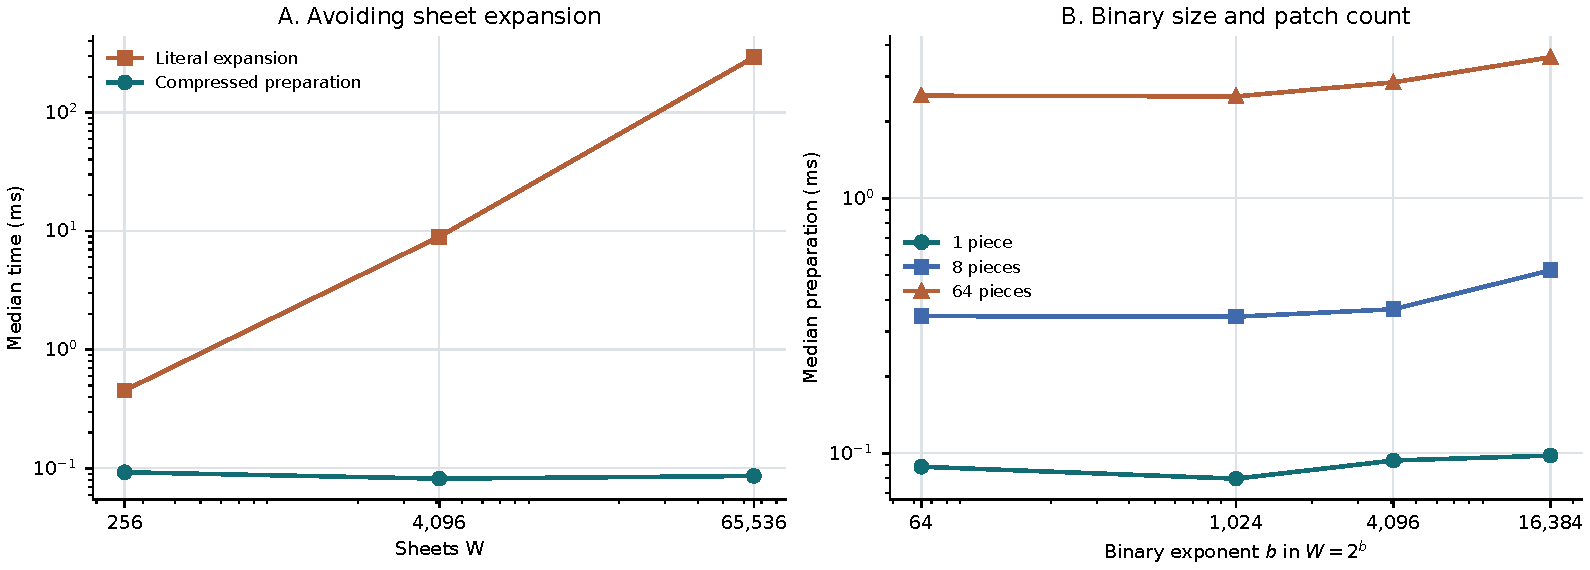
\includegraphics[width=\linewidth]{generated/geometry_scaling.pdf}
\caption{Measured preparation costs from the included raw data. Left: the
same annulus family at three explicit sheet counts, with the independent
expanded oracle. Right: compressed annulus chains as the binary exponent
and number of pieces vary. Connecting segments guide the eye; they are not
complexity fits.}
\label{fig:geometry}
\end{figure}

At $W=2^{16384}$ and 64 patches, median preparation is 3.571 milliseconds,
separate gauge-certificate replay is 1.283 milliseconds, and a prepared
32-mark query is 0.518 milliseconds. The summary serializes to 782,029
bytes and the marked signature to 494,410 bytes. These are compact relative
to $W$, but they are not constant-size outputs. The independent correctness
suite also exercises valid gluings at $W=2^{24000}$; that is an arithmetic
and topology test rather than a timed claim about recognition.

\subsection{Validation coverage and its limits}

The complete final repository suite ran 729 test methods in 102.519 seconds: 726 passed and 3 were skipped because they require the optional native Regina dependency. The pinned baseline had 697 methods and one error in the partial-input worker regression; that error is repaired. The final suite adds 32 methods: twelve primary, five integration, fourteen geometric, and one malformed-byte worker regression. The retained full log records all method names and the independent enumeration totals.


The twelve new primary test methods include exhaustive fixed-space checks
for every monic binary modulus of degrees one through six; independent
minimal-polynomial checks for all $2\times2$ binary matrices and seeded
$3\times3$ matrices; repeated factors; nilpotent and identity cases;
corrupted certificate rejection; cache separation; interruption; and exact
rank comparisons. A specific attachment test includes two different
matching types with recovered quantum shifts zero, one, and two, and checks
the complete change of basis. Existing scalar tests include 80 random
braid cases. Five integration tests exercise the exact and capped wrappers,
recognition and CLI dispatch, option rejection, and exhaustion semantics.

The fourteen new geometry test methods include 1,547 comparisons against
literal lifted surfaces and 6,216 ordered-mark comparisons against an
independent graph-action oracle. They cover boundary exhaustion, invalid
seams, reversed traversal, nonorientable pieces, closed outputs, alternative
valid gauge forests, corrupted certificate rejection, component and port
provenance, defensive copies, and immutable extension after failure.
The $W=1,2$ cases are included explicitly because written affine signs are
not faithful permutation labels there.

Finite tests do not prove the mathematics or substitute for independent
implementation review. Conversely, a proof about a model does not establish
that every line of code realizes it. The package supplies the proofs,
positive witness checks, small exhaustive comparisons, and a reproducible
complete repository suite as complementary evidence. Formal proof-assistant
verification remains a separate research task.

\section{What would actually imply quasipolynomial recognition?}
\label{sec:global}

\subsection{A composition bound with all size parameters visible}

Let $H(n)$ be the total number of examined global transitions, including
failed branches, hierarchy repairs, and rejected certificates. Let $P(n)$
bound the complete bit size of every live representation and operation
request: explicit scalar blocks and coefficient data, commutant equations,
surface pieces and attachment maps, binary multiplicities, curve or word
representations, and generated positive certificates. The maximum ranges
over every intermediate representation actually materialized, including
temporary expansions and the state before recompression. Let all local
work for one transition, including
construction, validation, lookup, output, and any required subroutine, be
bounded by $P(n)^c$ for a constant $c$.

\begin{proposition}[Conditional composition bound]
\label{prop:global}
Under these hypotheses, a correct complete recognition algorithm takes
\[
 T(n)\le\poly(n)+O\bigl(H(n)P(n)^c\bigr).
\]
If $\log H(n)$ and $\log P(n)$ are both
$O((\log(n+2))^2)$, this is $n^{O(\log n)}$.
More generally, quasipolynomial bounds on both $H$ and $P$ give a
quasipolynomial bound on $T$.
\end{proposition}
\begin{proof}
Charge each local operation, including its unsuccessful attempts, to the
transition performing it. By hypothesis the total charge per transition
is at most a constant times $P^c$. Summing gives the first expression.
Taking logarithms proves the remaining statements. Any subroutine lacking
the asserted bound is a missing hypothesis, not a term that may be omitted.
\end{proof}

This elementary proposition is useful because it exposes the actual gap.
Theorems~\ref{thm:assemblycost} and the polynomial-projector cost bound
justify some local charges. They do not bound the live scalar dimensions,
prove that geometric requests have the required affine form, or bound the
number of transitions. A local algorithm polynomial in an exponentially
large explicit matrix is still exponential in the original crossing count.
An algorithm polynomial in $\log W$ is more favorable when a large
multiplicity has remained genuinely binary throughout its construction.

A bounded heuristic that eventually falls back to complete Khovanov
scanning remains a valid recognizer when sufficient resources are allowed,
using the established unknot-detection theorem \cite{kronheimer-mrowka}.
For completeness, the coefficient bridge is as follows. For a knot $K$,
\[
 \dim_{\F}Kh(K;\F)=2\dim_{\F}\widetilde{Kh}(K;\F),
\]
by the characteristic-two splitting \cite[Corollary 3.2.C]{shumakovitch}.
Universal coefficients give
\[
 \dim_{\F}\widetilde{Kh}(K;\F)\ge
 \dim_{\mathbb Q}\widetilde{Kh}(K;\mathbb Q),
\]
and the latter is greater
than one for every nontrivial knot by the Kronheimer--Mrowka theorem.
The unknot has reduced rank one, so unreduced characteristic-two rank two
is equivalent to being the unknot.
That logical completeness does not improve its general exponential bound.
With fixed resource limits it is a sound partial recognizer whose
\code{UNKNOWN} outputs record precisely that distinction.

\subsection{Hierarchy depth, pattern complexity, and the exponent}

Suppose a hierarchy procedure has an iteration bound
\begin{equation}\label{eq:hierarchycount}
 H\le L(g+1)^L,
\end{equation}
as in the cited hierarchy framework, and suppose every iteration satisfies
the local cost hypothesis. Then
\begin{equation}\label{eq:exponentbudget}
 \log T\le O(\log n)+O(\log L)+L\log(g+1)+c\log P.
\end{equation}
The three terms involving $L,g,P$ have distinct mathematical origins.
Improving a normal-cut implementation does not automatically improve the
repair term $L\log(g+1)$.

\begin{center}
\begin{tabular}{llll}
\toprule
Hierarchy length $L$ & Pattern bound $g$ & Representation $P$ & Resulting bound\\
\midrule
$O(\log n)$ & $n^{O(1)}$ & $n^{O(1)}$ & $2^{O((\log n)^2)}$\\
$O((\log n)^2)$ & $n^{O(1)}$ & $n^{O(1)}$ & $2^{O((\log n)^3)}$\\
$O((\log n)^2)$ & $O(1)$ & $n^{O(1)}$ & $2^{O((\log n)^2)}$\\
\bottomrule
\end{tabular}
\end{center}
Each row is conditional on the complete per-iteration accounting. The last
row points to an alternative to reducing hierarchy depth: sufficiently
strong control of the pattern choices could achieve the sharper exponent
at the same depth. No such uniform pattern bound is proved here.

The geometric kernel helps with a specific part of $P$ and its local cost.
A parallelity region represented as checked dihedral cover pieces can be
sewn and queried without replacing a binary degree by that many explicit
components. To use this fact in~\eqref{eq:exponentbudget}, one must still
extract the pieces and seams from the embedded normal-cut data and prove
closure of the representation under every subsequent operation. The
compressed-cut theorem in the 2026 preprint is a significant relevant
input; it does not by itself discharge all of Section 9's operation costs
\cite{lackenby-hierarchy}.

\subsection{A sharper sufficient condition for variable lexicographic bounds}

A single worst-case $g$ can hide useful variation between hierarchy levels.
Suppose the progress measure is a fixed-length vector with coordinate
bounds $0\le x_i\le G_i$ that apply uniformly throughout every examined
history, and each macrostep strictly decreases its lexicographic value.
Coordinates are padded consistently so that
changing hierarchy length does not evade the order. Then the number of
possible values is at most
\[
 \prod_{i=1}^{L}(G_i+1).
\]
If at most $F(n)$ charged operations occur between consecutive decreases,
including initialization and termination, then
$H(n)\le F(n)\prod_i(G_i+1)$. The relevant exponent budget, in addition to
$\log F(n)$, is therefore
\begin{equation}\label{eq:weightedbudget}
 \sum_{i=1}^{L}\log(G_i+1),
\end{equation}
rather than just the largest coordinate or the length of the written
vector.

For example, proving~\eqref{eq:weightedbudget} to be
$O((\log n)^2)$ would suffice for the sharper target when $P$ and the
per-value factor satisfy the same logarithmic bound. A small binary
encoding of a decreasing integer does not alone imply few transitions:
a $b$-bit counter may still take $2^b$ distinct values. Equally, decreasing
one coordinate while allowing lower coordinates to reset is sound only
when their complete ranges remain bounded. These are explicit obligations
for a proposed amortized hierarchy proof.

\subsection{Algebraic state sharing has a corresponding obstruction}

The same accounting applies to compressed Khovanov states. Splitting a
component may expose repeated templates and reduce later operations, but
it may also leave object counts unchanged, as the measured examples do.
A theorem would need a bound on the number and size of distinct live
templates, the bit lengths of their multiplicities and grading data, and
the cost of updating all attachments as crossings are added. Neither
semisimplicity of a chosen commutative subalgebra nor a successful split at
one stage bounds those quantities at the next stage.

The two-field construction also warns against treating candidate behavior
as universal. Uniform random field values give the favorable probability
in Theorem~\ref{thm:probability}; repeated isomorphic primary factors can
make every polynomial in one candidate fail to distinguish certain
summands. A general representation theorem or a genuinely broader
endomorphism algorithm is needed before assigning a global asymptotic
benefit to this optional kernel.

\subsection{A concrete next optimization: reuse the corner algebras}

The complete-compression measurements suggest a specific improvement that
has a short exact justification. Let $R=\End^0_{\mathrm{scalar}}(C)$ be the
complete typed scalar chain-endomorphism algebra, and let
$1=e_1+\cdots+e_s$ be pairwise orthogonal typed scalar idempotents giving a
verified decomposition $C=\bigoplus_i C_i$ with the inherited scalar types.

\begin{proposition}[Transported corner spaces]
\label{prop:corners}
There are natural identifications
\[
 \End^0_{\mathrm{scalar}}(C_i)\cong e_i R e_i,
 \qquad
 R=\bigoplus_{i,j}e_i R e_j
 \quad\text{as vector spaces}.
\]
In particular, a complete vector-space basis $R_1,\ldots,R_a$ of $R$
provides spanning sets $\{e_iR_j e_i:1\le j\le a\}$ for all child
commutants, and
\[
 \sum_i\dim_{\F}\End^0_{\mathrm{scalar}}(C_i)\le\dim_{\F}R.
\]
\end{proposition}
\begin{proof}
Write the inclusion and projection of $C_i$ as $u_i,v_i$, so that
$u_iv_i=e_i$ and $v_iu_i=1$. A typed scalar endomorphism $a$ of $C_i$
extends to $u_iav_i\in R$ supported on that summand. Conversely, restricting
$e_i r e_i$ gives $v_i r u_i$. These maps are inverse and preserve
multiplication. Every $r\in R$ equals $\sum_{i,j}e_i r e_j$; multiplying a
linear relation on the left and right by chosen idempotents proves that
this sum of subspaces is direct. The dimension inequality follows by
retaining only diagonal terms.
\end{proof}

Thus a static decomposition pass need not solve the original differential
commutation equations afresh for every child. It can conjugate and restrict
the already computed basis, discard linear dependencies, and pass the
resulting corner basis down the decomposition tree. This is an application
of a standard corner-algebra identity, not a new structural theorem about
finite-dimensional algebras. Its value here is that it isolates a reusable
object that the current implementation discards.

The inequality gives an amortized \emph{dimension} budget at every frontier
of a static refinement tree. Every nonzero child has a nonzero identity,
so a proper refinement tree has at most $a$ leaves; it also has at most
$D$ leaves by total scalar dimension. If each internal node has at least
two nonzero children, there are at most $\min(a,D)-1$ internal refinements.
A simultaneous conjugation of $a$ explicit $D$-dimensional basis matrices
by the splitting basis and its inverse costs $O(aD^3)$ binary operations;
all child matrices are then restrictions of the conjugated matrices.
At any depth the child commutant dimensions
sum to at most $a$, so total basis-conjugation work over the accepted
static tree is bounded by $O(aD^3\min(a,D))$, hence $O(aD^4)$.
Candidate search, dependency elimination, and differential-attachment
transport are additional costs. Alternative or backtracking trees are
also outside this particular bound.
Simultaneous primary refinement can reduce the number of separate
transports. This optimization is proposed and proved at the interface
level, but is not implemented or included in the reported speed figures.

Adding a crossing or changing the differential invalidates the simple
static argument. Reusing a corner basis through those mutations requires a
new exact update rule or a fresh solve. The first implementation should
therefore target one existing \code{_compress} call, where the benchmark
exhibits repeated child solves as an explicit operation to profile.

\section{Proposed research questions and work program}
\label{sec:research}

The following questions are ordered by their relation to the demonstrated
kernels and to the eventual recognition theorem. Each has a specific
mathematical or experimental deliverable. They should be treated as open
work items, not as assumptions already validated by this article.

\subsection{Near-term algebraic questions}

\paragraph{1. Can corner reuse turn successful splitting into a full-pass gain?}
Implement Proposition~\ref{prop:corners} inside one static compression pass.
Retain the original complete commutant basis, transport it through every
accepted basis change, and derive child bases by corner restriction and
independent elimination. Compare identical decompositions, complete wall
clock, transported matrix volume, and peak memory. A successful result
would preserve the current witness checks while reducing complete-pass
cost on $r=8,10$ without a comparable regression on the bridge and natural
controls. The proposed optimization should first be tested with the same
canonical commutant bases or a replay of the same candidates in both arms.
Merely fixing the policy does not control candidate changes caused by a
different input basis.

\paragraph{2. Which trigger policy makes primary discovery worthwhile?}
A primary candidate may be cheap to reject or expensive to analyze, and
the old basis order can already expose easy idempotents. Develop a cost
model using block sizes, estimated minimal-polynomial degree, remaining
split allowance, and the measured cost of a commutant solve. Compare
immediate fallback, delayed fallback after the ordinary candidate pass,
and shared power tables. This is an algorithm-selection problem, not a
license to omit unfavorable cases. Record primary invocations, positive
splits, failed-call time, child-solve time, and total recognition time.

\paragraph{3. Can all polynomial summands be extracted in one certified pass?}
Use a basis of the Berlekamp algebra to refine idempotents by $e\mapsto ep$
and $e\mapsto e(1+p)$, removing zero pieces. Berlekamp's classical argument
identifies all primary factors of the chosen cyclic algebra. The new task
is to obtain one combined typed basis change, retain grading and all
attachments, and compare its matrix-transport cost with recursive binary
splitting. This remains incomplete for the full noncommutative commutant,
so the output contract must say exactly which family of projectors was
exhausted.

\paragraph{4. Can the comparison family occur in genuine knot computations?}
Determine whether the connected $xI+yA$ family, or a comparable family with
the same scalar endomorphism obstruction, occurs as a reduced prefix of a
classical knot diagram under the repository's exact scanner. A proof of
realizability would connect the candidate separation to the target domain.
A proof of impossibility would be equally informative: it could reveal
relations satisfied by reachable prefixes that generic category objects
miss. Finite searches should retain the original diagram, crossing order,
all basis changes, and a replayable provenance chain. Merely finding an
isomorphic matrix after deleting external attachments is insufficient.

\paragraph{5. What can replace polynomial-in-one-operator search?}
Repeated primary types are invisible to one cyclic subalgebra. Study the
semisimple quotient and radical of the full typed scalar commutant, or
several interacting candidates, with explicit field and bit costs. A useful
target is a deterministic decomposition routine whose accepted idempotents
have the same small positive certificates as the present backend. One
must not linearize $Q\mapsto Q^2+Q$ on a noncommutative algebra: the cross
terms make that map nonlinear. Every use of Frobenius linear algebra must
identify its commutative domain.

\paragraph{6. Is there a size theorem for reachable shared states?}
Seek structural bounds on distinct templates, template dimensions,
multiplicity bit lengths, and attachment complexity after each crossing.
A bound on boundary width alone does not bound arbitrary multiplicity
spaces unless the representation theorem explicitly says so. Start with
restricted families such as controlled braid width or bounded separator
profiles and state the dependence on each parameter. The decisive outcome
would be a bound strong enough for Proposition~\ref{prop:global}, not only
smaller constants on a fixed corpus.

\subsection{Geometric representation and attachment questions}

\paragraph{7. Can real normal cuts produce checked seam presentations?}
Implement an extractor from a triangulation or uniform-type handle
structure and compressed normal coordinates to the piece/seam input of
Section~\ref{sec:seam-input}. The extractor must derive peripheral words,
local orientations, fibre coordinates, and seam maps from the actual
embedded construction. Its certificate must connect the abstract cover to
the cut manifold's attaching data. First establish a restricted theorem
for a recognizable dihedral parallelity configuration; reject inputs
outside that class. Guessing an affine action from component counts would
lose the information highlighted by Example~\ref{ex:klein}.

\paragraph{8. How far can the full-boundary promise be relaxed?}
Normal-surface orbit systems can involve partial intervals and multiple
coordinate ranges. Investigate whether such data admit a bounded number
of signed-affine charts, or require the more general interval-pairing
machinery. A precise extension should state its allowed breakpoints,
binary coordinate lengths, chart overlap maps, and composition rule.
Measure complexity before normalizing or refining all charts. Prove a
bound on newly introduced breakpoints; otherwise avoiding sheet expansion
can simply move the exponential growth into the number of intervals.

\paragraph{9. Can seam insertion be maintained incrementally?}
The present immutable extension reconstructs its index. A dynamic version
could maintain affine potentials on a disjoint-set forest, with new cycle
generators updating gcd and orientation data. The difficulty is preserving
all old piece coordinates, component labels, fixed-residue exceptions,
boundary availability, and ordered-mark queries when components merge.
A useful theorem would give an amortized bit bound including large-integer
arithmetic and the cost of emitted updates. Returning a full changed
summary after each insertion still costs its full output size.

\paragraph{10. Which embedded attachment queries are sufficient for hierarchy repair?}
Point and boundary-lift labels are only part of a 3-manifold boundary
pattern. Identify the exact queries used by the hierarchy's repair steps:
for example, curve isotopy, intersection, relative position, product-region
attachment, and the distinction between compressible and essential
patterns. Relate them to compressed surface-curve algorithms such as
Lackenby's normal-curve procedures \cite{lackenby-curves}. The main issue is
constructing their required inputs with controlled length while preserving
embedding provenance. An abstract homeomorphism type and a list of marked
points do not by themselves solve these questions.

\subsection{Global complexity and research infrastructure}

\paragraph{11. Can hierarchy progress satisfy a total logarithmic budget?}
For an explicit hierarchy algorithm, identify the actual progress vector,
its coordinate ranges, and every transition that changes it. Prove either
a bound on $L\log(g+1)$ or the more precise sum in
\eqref{eq:weightedbudget}. Investigate whether geometric simplification
reduces the number of genuinely variable pattern choices at most levels.
A logarithmic depth bound, a constant pattern bound, and a weighted
coordinate bound are different routes with different proof obligations.
Adopt the exponent ledger~\eqref{eq:exponentbudget} before optimizing an
individual subroutine, so each improvement has a visible global role.

\paragraph{12. Which hard instances exercise the new operations?}
Build a versioned corpus that separates filter exits, ordinary scalar
splits, active primary failures, active primary successes, large affine
cover degrees, and normal-cut extraction failures. Include hard unknot
presentations and knotted controls with weak classical invariants, and
retain exact input diagrams and generation histories. Transforming one
knot diagram many times should not be confused with sampling independent
knot types. Report per-family results and unfavorable tails, rather than
a single aggregate speed factor. Search-generated witnesses should be
frozen before comparing new trigger policies.

\paragraph{13. What should a small independently trusted checker verify?}
Specify a certificate language for scalar decompositions and geometric
attachments. For algebra, the positive projector and conjugation checks
already provide a starting point; a complete commutant-basis certificate
would additionally need rank/completeness evidence. For geometry, extend
the gauge certificate with the normal-cut extraction witness rather than
trusting a serialized genus. Formalize the small algebraic and covering
lemmas in the proof system used by the repository, with exact treatment of
binary integers, $W=1,2$, orientation characters, and interruption states.
The current Python tests and prose proofs are not machine-checked formal
proofs.

\paragraph{14. Can a portfolio retain a proved worst-case bound?}
A practical recognizer may combine cheap filters, Khovanov methods, and a
geometric hierarchy. To inherit a future quasipolynomial theorem, give the
proved branch a fair, quantitatively bounded share of resources and charge
all speculative work. An unbounded heuristic performed first can destroy
a worst-case guarantee even when a good fallback exists. Conversely,
bounded optional algebraic work can coexist with a proved geometric bound.
The scheduling theorem must include preprocessing, subprocess startup,
certificate checking, and the cost of converting between representations.

\subsection{Suggested order of work}

The most concrete implementation step is corner reuse, followed by a
controlled comparison of primary trigger policies. The most consequential
geometric step is a certified extractor on a restricted real normal-cut
family. Those projects can proceed independently and share a common
witness and benchmark discipline. A global asymptotic claim should wait
for explicit representation-closure and progress bounds; the local proofs
in this article can then be inserted as established subroutines rather
than rediscovered during the global argument.

\section{Reproduction and repository integration}
\label{sec:reproduce}

The accompanying archive is intended to be reviewed and integrated at the
pinned baseline. It contains the article source and PDF, generated tables
and figure, the complete relevant source snapshot, the required historical
test oracles, raw numerical evidence, validation logs, a baseline patch,
and file hashes. Historical benchmark-result directories unrelated to this
continuation are omitted from the snapshots; the test fixtures and source
files needed by the maintained suite are retained.

The source snapshot is under \code{source/Topology/UnknotRecognition/}.
The \code{fast} directory remains a normal standalone Python package.
The historical \code{reports/24/reference}, \code{reports/26/detshadow},
and \code{reports/28/src} modules are retained because existing tests import
them. Their presence is a reproduction dependency, not a claim that their
older results are new contributions.

\begin{lstlisting}[language=bash]
# Run from the extracted archive root.
python scripts/reproduce.py --verify
python scripts/reproduce.py --tests
python scripts/make_figures.py
cd article
pdflatex -interaction=nonstopmode -halt-on-error unknot_projectors_and_seams.tex
pdflatex -interaction=nonstopmode -halt-on-error unknot_projectors_and_seams.tex
\end{lstlisting}

The verification command checks archive hashes and the recorded measured
source hashes. The test command runs the complete maintained suite from
the packaged source. Benchmarks are opt-in because their runtime is
substantially longer than a single example:

\begin{lstlisting}[language=bash]
python scripts/reproduce.py --benchmarks
# Individual operations, from source/.../fast:
python -m fastunknot recognize examples/trefoil.json --backend primary
python -m fastunknot khovanov examples/trefoil.json --primary
python -m fastunknot.surface_gluing gluing_research/examples/torus_twenty.json
\end{lstlisting}

The fresh benchmark files use a separate output directory and do not
replace the retained measurements. Wall-clock samples will vary by
machine. The geometry driver's metadata collection has a small portability
change after the measured run: outside a Git checkout it now records a
null commit instead of failing. The exact measured driver is retained
under \code{evidence/measured_sources}; the arithmetic kernels and timed
operations are unchanged. This distinction is explicit in the source
manifest.

The integration patch contains both new kernels, public dispatch, tests,
research fixtures and drivers, and the carried-forward worker repair with
the additional malformed-byte regression. Apply it only after checking the
baseline or resolving later repository changes. The package's baseline
snapshot permits a local patch-application check without a network fetch.
The supplied article is a research continuation with proved restricted
results and documented open problems; it is not a completed general
quasipolynomial recognition proof.

\begin{thebibliography}{20}

\bibitem{repo}
Vladimir Reshetnikov and contributors.
\emph{ProveIt: Topology/UnknotRecognition}, repository source and maintained
research synthesis, commit
\code{bc5b913850f78155ccfddd808d4b11517dca252d}.
\url{https://github.com/VladimirReshetnikov/ProveIt/tree/bc5b913850f78155ccfddd808d4b11517dca252d/Topology/UnknotRecognition}.
Accessed 8 October 2026.

\bibitem{berlekamp}
Elwyn R. Berlekamp.
Factoring polynomials over finite fields.
\emph{Bell System Technical Journal} 46(8) (1967), 1853--1859.
\url{https://doi.org/10.1002/j.1538-7305.1967.tb03174.x}.
Author's overview:
\url{https://math.berkeley.edu/~berlek/poly.html}.

\bibitem{hatcher}
Allen Hatcher.
\emph{Algebraic Topology}. Cambridge University Press, 2002.
Section 1.3, covering spaces and monodromy.
\url{https://pi.math.cornell.edu/~hatcher/AT/AT.pdf}.

\bibitem{aht}
Ian Agol, Joel Hass, and William Thurston.
The computational complexity of knot genus and spanning area.
\emph{Transactions of the American Mathematical Society} 358(9) (2006),
3821--3850.
\url{https://arxiv.org/abs/math/0205057}.

\bibitem{kronheimer-mrowka}
Peter B. Kronheimer and Tomasz S. Mrowka.
Khovanov homology is an unknot-detector.
\emph{Publications Math\'ematiques de l'IH\'ES} 113 (2011), 97--208.
\url{https://arxiv.org/abs/1005.4346}.

\bibitem{shumakovitch}
Alexander N. Shumakovitch.
Torsion of Khovanov homology.
\emph{Fundamenta Mathematicae} 225 (2014), 343--364.
Corollary 3.2.C.
\url{https://doi.org/10.4064/fm225-1-16}.

\bibitem{lackenby-talk}
Marc Lackenby.
\emph{Unknot recognition in quasi-polynomial time}.
Oxford lecture handout, March 2021, 34 slides; in particular slides 7 and 25.
\url{https://people.maths.ox.ac.uk/lackenby/quasipolynomial-talk-oxford-compressed.pdf}.

\bibitem{lackenby-hierarchy}
Marc Lackenby.
\emph{Incompressible surfaces, hierarchies and unknot recognition}.
Preprint, arXiv:2607.23350v1, July 2026.
In particular Section 9, Proposition 9.1, and Theorem 14.4.
\url{https://arxiv.org/html/2607.23350v1}.

\bibitem{lackenby-curves}
Marc Lackenby.
\emph{Some fast algorithms for curves in surfaces}.
Author's manuscript, 13 January 2026.
\url{https://people.maths.ox.ac.uk/lackenby/AlgorithmsSurfaces13jan26.pdf}.

\end{thebibliography}
\end{document}
